\section{Marco conceptual}
\label{sec:marco_conceptual}
En esta sección se presentan conceptos y bases teóricas respecto a la temática que conduce el desarrollo de este trabajo, el cual tiene relación con el uso de interfaces no tradicionales, específicamente con una interfaz operada con el cuerpo. Además, se indaga sobre ciertas definiciones para establecer lo que se pretende medir en este estudio, lo que involucra la experiencia de usuario y métricas de rendimiento en la realización de tareas. Finalmente, se proponen ciertas características fundamentales respecto de este tipo de proyectos relacionados con diseños experimentales con usuarios.

\subsection{Recuperación de Información Humano Computador}
\label{subsec:HCIR}
La Recuperación de Información Humano Computador\footnote{Traducción libre.} (HCIR, por sus iniciales en inglés de \ingles{Human Computer Information Retrieval}) es el estudio de los métodos que integran la inteligencia humana y la búsqueda algorítmica para ayudar a la gente a mejorar la búsqueda, exploración y aprendizaje de información \parencite{marchionini2006}. Dentro de esta área interactúan otras disciplinas, como la recuperación de información, llamada en inglés \ingles{Information Retrieval} (IR), la que está enfocada principalmente en proveer a los usuarios de fácil acceso a la información de su interés trabajando con la representación, almacenamiento, organización y acceso a objetos de información como documentos, páginas \ingles{web}, catálogos en línea y objetos multimedia \parencite{ricardo2011modern} y la búsqueda de información, llamada en inglés \ingles{Information Seeking} (IS) que se entiende como un proceso más orientado al usuario y abierto que IR. En IS, no se sabe si existe una respuesta a la consulta del usuario, por lo que el proceso de búsqueda puede proporcionar el aprendizaje necesario para satisfacer su necesidad de información \parencite{ricardo2011modern}.

La búsqueda de información es un campo de la investigación que relaciona el desarrollo del área de las tecnologías y ciencias de la computación con la psicología y ciencias sociales en el procesamiento de la información, en donde el usuario toma un papel activo por medio de interacciones explicitas e implícitas con la información \parencite{carroll1997human}. Es una disciplina que contempla tanto al sistema como al usuario, así como la relación que se establece a través del comportamiento del usuario y sus experiencias \parencite{kelly2009methods}. Se ubica en un punto medio entre las disciplinas de HCI e IR.

\subsection{Rendimiento}
\label{subsec:rendimiento}
En el contexto de la recuperación de información se definen \ingles{precision} y \ingles{recall} en función de un conjunto de documentos relevantes y un conjunto de documentos recuperados \parencite[p.~38]{powers2011evaluation}, las cuales se definen a continuación.  

\begin{description}
	\item [\ingles{Precision}] Métrica que mide la razón de documentos relevantes recuperados con 
respecto al total de documentos recuperados. Representado en la \eq{eq:precision}, el resultado de esta métrica es un valor continuo entre 0 y 1, mientras más cercano a 1, mayor fue su precisión al encontrar los documentos relevantes.

	\begin{equation}
	Precision = \frac{\big[\big\{documentos \ relevantes\big\} \cap \big\{documentos \ recuperados\big\}\big]}{\big\{documentos \ recuperados\big\}}
	\label{eq:precision}
	\end{equation}

	\item [\ingles{Recall}] Métrica que mide la razón de documentos relevantes recuperados con 
respecto al total de documentos relevantes. Representado en la \eq{eq:recall}, el resultado de esta métrica es un valor continuo entre 0 y 1, mientras más cercano a 1, mayor fue la recuperación de documentos en base al total del universo disponible.

	\begin{equation}
	Recall = \frac{\big[\big\{documentos \ relevantes\big\} \cap \big\{documentos \ recuperados\big\}\big]}{\big\{documentos \ relevantes\big\}}
	\label{eq:recall}
	\end{equation}

	\item [\ingles{F1}] Métrica que considera los valores de \ingles{precision} y \ingles{recall} en un promedio ponderado. Representado en la \eq{eq:F1}, el resultado de esta métrica es un valor continuo entre 0 y 1, en que un valor cercano a uno permite identificar a los estudiantes con una recuperación de documentos proporcional a su precisión, respecto a la relevancia de estos.  

	\begin{equation}
	F1 = \frac{2 \cdot Precision\cdot Recall}{Precision+ Recall}
	\label{eq:F1}
	\end{equation}
 
\end{description}

%\begin{equation}
%	Precision = \frac{TP}{TP+ FP}
%\end{equation}
%\begin{equation}
%	Recall = \frac{TP}{TP+ FN}
%\end{equation}
\subsection{Alfabetización informacional}
\label{subsec:alfabetizacion}
La alfabetización informacional (conocida en inglés como \ingles{information literacy}) es definida como “el grupo de habilidades en las que se requiere reconocer cuándo la información es necesaria y tener la habilidad de encontrar, evaluar y usar efectivamente dicha información necesaria” \footnote{\traduccionlibre} \parencite[p.~2]{american2000information}. Es un campo que cubre varias áreas, entre las que se destaca la alfabetización digital, las habilidades de uso de bibliotecas, la ética informacional, la lectura crítica, el pensamiento crítico, los derechos de autor, la seguridad y privacidad, entre otras. A través del estudio de estas áreas como factores que influyen a la alfabetización informacional se puede obtener una visión clara de cómo los estudiantes llevan a cabo sus tareas de obtención y selección de información.

\subsection{Competencias de investigación en línea}
\label{subsec:competencias}
Se definen las competencias de investigación (\ingles{inquiry skills}, por su nombre en inglés) como “las habilidades para explorar preguntas, para poder reunir, interpretar y sintetizar diferentes tipos de información y datos, además de desarrollar y compartir una explicación para responder preguntas dadas” \footnote{\traduccionlibre} \parencite[p.~13]{national2000inquiry}. En base a este concepto nacen las competencias de investigación en línea (conocidas en inglés como \ingles{online inquiry skills}), que son una instancia específica de las competencias de investigación, pero aplicada sobre información disponible en línea \parencite{quintana2005framework}.

Las competencias de investigación en línea involucran una serie de actividades cognitivas, como generar una pregunta de investigación, buscar información relevante en colecciones digitales, evaluar y seleccionar la información encontrada, e integrar coherentemente la información seleccionada para responder la pregunta original \parencite{eisenberg1990information}.

\subsection{Aprendizaje automático}
El aprendizaje automático (\ingles{machine learning}, por su nombre en inglés) es un área de la Inteligencia Artificial enfocada al desarrollo de algoritmos capaces de generalizar comportamientos, a partir de información no estructurada suministrada en forma de ejemplos, de manera que posean la capacidad de adaptarse en base a experiencia adquirida y no deban ser reprogramados. Los diversos algoritmos de esta rama se diferencian en su forma de llevar a cabo el aprendizaje, algunas de estas son:

\begin{description}
\item [Aprendizaje supervisado] Se realiza mediante un entrenamiento controlado por un agente externo (supervisor, maestro), que determina la respuesta que se debería generar a partir de una entrada determinada. El supervisor controla la salida y en caso de que esta no coincida con la deseada. Se modifican los parámetros usados, con el fin de conseguir que la salida obtenida se aproxime a la deseada.

\item [Aprendizaje no supervisado] Se realiza mediante un entrenamiento sin conocimiento a priori de la salida deseada, es decir, solo son conocidas las entradas, por lo tanto el aprendizaje se basa en el grado de familiaridad o similitud entre la información que presenta una entrada y la información recolectada por entradas anteriores.
\end{description}

Uno de los problemas que intenta solucionar la rama de aprendizaje automático supervisado, es la clasificación, cuya definición en este contexto corresponde al problema de identificar a qué categoría pertenece una nueva observación. 

Un clasificador se define como cualquier algoritmo que resuelva el problema de clasificación. Para ello, este tipo de algoritmo necesita ser entrenado con un conjunto de observaciones que ya estén etiquetadas en una categoría, de forma que pueda corregir su aprendizaje. Las observaciones son representadas a través de un conjunto de propiedades que permiten determinar a qué categoría pertenece. Por su parte, las propiedades pueden ser de tipo categórico (por ejemplo el tipo de sangre), ordinal (“grande”, “medio”, “pequeño”), valores enteros o reales o incluso utilizando la diferencia y similitud entre la observación actual y las observaciones previas (Vilches, 2015). Como consecuencia del entrenamiento, se consigue un modelo del clasificador capaz de asignar observaciones desconocidas a una categoría conocida específica, solo sabiendo sus propiedades.

La terminología usada en esta área, suele llamar a las observaciones “instancias”, “ejemplos” o “sujetos”, a las propiedades “características” o “atributos”, a las categorías “clases”, al conjunto de observaciones “conjunto de entrada” y al conjunto de observaciones usadas en el entrenamiento “conjunto de entrenamiento”.


Debido a las características de este proyecto, se utilizan técnicas de aprendizaje automático supervisado.

\subsection{Técnicas de aprendizaje automático supervisado}
\label{subsec:tecnicas-mineria}
A continuación, se describen los algoritmos y datos seleccionados para esta investigación.

\subsubsection*{Árboles de decisión}

\begin{figure}[H]
	\centering
	\newdimen\nodeDist
\nodeDist=35mm

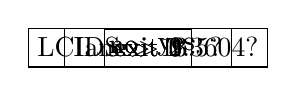
\begin{tikzpicture}[
    node/.style={%
      draw,
      rectangle,
    },
  ]

    \node [node] (A) {IDS $>$ 13.5?};
    \path (A) ++(-135:\nodeDist) node [node] (B) {exit 1};
    \path (A) ++(-45:\nodeDist) node [node] (C) {LCIanx $>$ 0.3604?};
    \path (C) ++(-135:\nodeDist) node [node] (D) {exit 2};
    \path (C) ++(-45:\nodeDist) node [node] (E) {exit 3};

    \draw (A) -- (B) node [left,pos=0.25] {no}(A);
    \draw (A) -- (C) node [right,pos=0.25] {yes}(A);
    \draw (C) -- (D) node [left,pos=0.25] {no}(A);
    \draw (C) -- (E) node [right,pos=0.25] {yes}(A);
\end{tikzpicture}
	\captionsource{Árbol de decisión}{\fuentePropia}
	\label{fig:decision-tree}
\end{figure}


\subsubsection*{Máquinas de vectores de soporte (SVM)}
Las máquinas de vectores de soporte o SVM (del inglés \ingles{Support Vector Machine}) son un conjunto de algoritmos de aprendizaje supervisado que se enfocan en resolver problemas de clasificación, regresión y agrupamiento. La SVM destinada para clasificación, es un clasificador lineal binario que busca encontrar un hiperplano que separe de forma óptima un conjunto de datos, maximizando la distancia entre las dos clases.


\begin{figure}[H]
	\centering
	\begin{tikzpicture}[&gt;=stealth']
  % Draw axes
  \draw [&lt;-&gt;,thick] (0,5) node (yaxis) [above] {$y$}
        |- (5,0) node (xaxis) [right] {$x$};
  % draw line
  \draw (0,-1) -- (5,4); % y=x-1
  \draw[dashed] (-1,0) -- (4,5); % y=x+1
  \draw[dashed] (2,-1) -- (6,3); % y=x-3
  % \draw labels
  \draw (3.5,3) node[rotate=45,font=\small] 
        {$\mathbf{w}\cdot \mathbf{x} + b = 0$};
  \draw (2.5,4) node[rotate=45,font=\small] 
        {$\mathbf{w}\cdot \mathbf{x} + b > 1$};
  \draw (4.5,2) node[rotate=45,font=\small] 
        {$\mathbf{w}\cdot \mathbf{x} + b < -1$};
  % draw distance
  \draw[dotted] (4,5) -- (6,3);
  \draw (5.25,4.25) node[rotate=-45] {$\frac{2}{\Vert \mathbf{w} \Vert}$};
  \draw[dotted] (0,0) -- (0.5,-0.5);
  \draw (0,-0.5) node[rotate=-45] {$\frac{b}{\Vert \mathbf{w} \Vert}$};
  \draw[-&gt;] (2,1) -- (1.5,1.5);
  \draw (1.85,1.35) node[rotate=-45] {$\mathbf{w}$};
  % draw negative dots
  \fill[red] (0.5,1.5) circle (3pt);
  \fill[red]   (1.5,2.5)   circle (3pt);
  \fill[black] (1,2.5)     circle (3pt);
  \fill[black] (0.75,2)    circle (3pt);
  \fill[black] (0.6,1.9)   circle (3pt);
  \fill[black] (0.77, 2.5) circle (3pt);
  \fill[black] (1.5,3)     circle (3pt);
  \fill[black] (1.3,3.3)   circle (3pt);
  \fill[black] (0.6,3.2)   circle (3pt);
  % draw positive dots
  \draw[red,thick] (4,1)     circle (3pt); 
  \draw[red,thick] (3.3,.3)  circle (3pt); 
  \draw[black]     (4.5,1.2) circle (3pt); 
  \draw[black]     (4.5,.5)  circle (3pt); 
  \draw[black]     (3.9,.7)  circle (3pt); 
  \draw[black]     (5,1)     circle (3pt); 
  \draw[black]     (3.5,.2)  circle (3pt); 
  \draw[black]     (4,.3)    circle (3pt); 
\end{tikzpicture}
	\captionsource{SVM}{\fuentePropia}
	\label{fig:svm}
\end{figure}

\subsubsection*{Perceptrón}

\begin{figure}[H]
	\centering
	% Multilayer perceptron
\usetikzlibrary{positioning}

\tikzstyle{inputNode}=[draw,circle,minimum size=10pt,inner sep=0pt]
\tikzstyle{stateTransition}=[-stealth, thick]

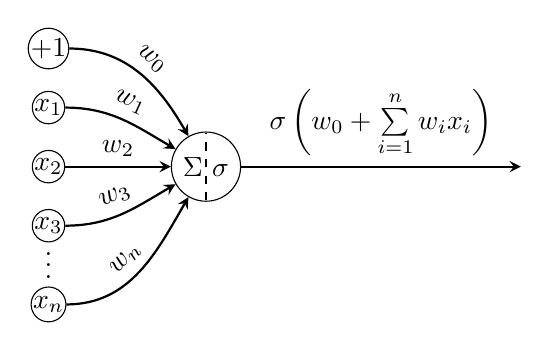
\begin{tikzpicture}
    \node[draw,circle,minimum size=25pt,inner sep=0pt] (x) at (0,0) {$\Sigma$ $\sigma$};

    \node[inputNode] (x0) at (-2, 1.5) {$\tiny +1$};
    \node[inputNode] (x1) at (-2, 0.75) {$\tiny x_1$};
    \node[inputNode] (x2) at (-2, 0) {$\tiny x_2$};
    \node[inputNode] (x3) at (-2, -0.75) {$\tiny x_3$};
    \node[inputNode] (xn) at (-2, -1.75) {$\tiny x_n$};

    \draw[stateTransition] (x0) to[out=0,in=120] node [midway, sloped, above] {$w_0$} (x);
    \draw[stateTransition] (x1) to[out=0,in=150] node [midway, sloped, above] {$w_1$} (x);
    \draw[stateTransition] (x2) to[out=0,in=180] node [midway, sloped, above] {$w_2$} (x);
    \draw[stateTransition] (x3) to[out=0,in=210] node [midway, sloped, above] {$w_3$} (x);
    \draw[stateTransition] (xn) to[out=0,in=240] node [midway, sloped, above] {$w_n$} (x);
    \draw[stateTransition] (x) -- (4,0) node [midway,above] {$\sigma\left(w_0 + \sum\limits_{i=1}^{n}{w_ix_i}\right)$};
    \draw[dashed] (0,-0.43) -- (0,0.43);
    \node (dots) at (-2, -1.15) {$\vdots$};
    
\end{tikzpicture}

	\captionsource{Perceptrón}{\fuentePropia}
	\label{fig:perceptron}
\end{figure}

\begin{equation}
 \pmb{\mu_1} = \begin{bmatrix}0\\0\\...\\0\end{bmatrix}
\end{equation}

\subsubsection*{Perceptrón multicapa}

\begin{figure}[H]
	\centering
	% Multilayer perceptron
\usetikzlibrary{positioning}

\tikzstyle{inputNode}=[draw,circle,minimum size=10pt,inner sep=0pt]
\tikzstyle{stateTransition}=[-stealth, thick]

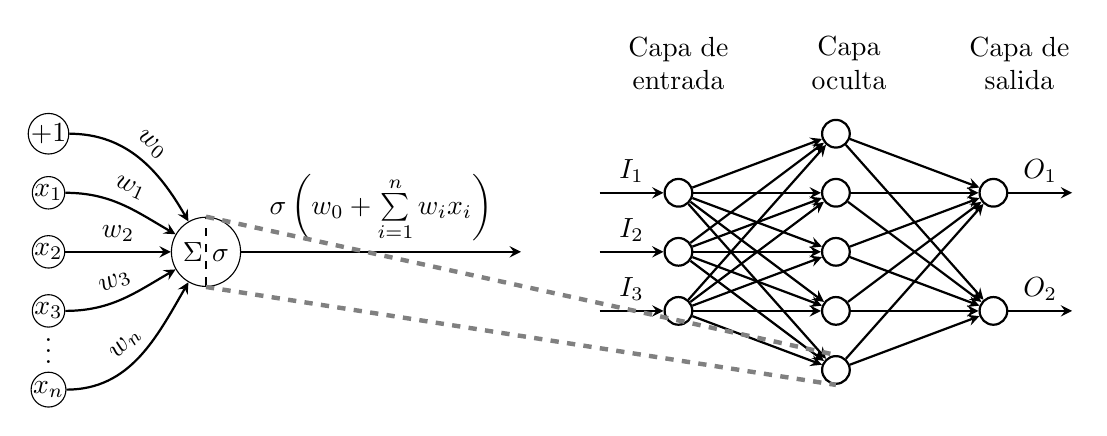
\begin{tikzpicture}
    \node[draw,circle,minimum size=25pt,inner sep=0pt] (x) at (0,0) {$\Sigma$ $\sigma$};

    \node[inputNode] (x0) at (-2, 1.5) {$\tiny +1$};
    \node[inputNode] (x1) at (-2, 0.75) {$\tiny x_1$};
    \node[inputNode] (x2) at (-2, 0) {$\tiny x_2$};
    \node[inputNode] (x3) at (-2, -0.75) {$\tiny x_3$};
    \node[inputNode] (xn) at (-2, -1.75) {$\tiny x_n$};

    \draw[stateTransition] (x0) to[out=0,in=120] node [midway, sloped, above] {$w_0$} (x);
    \draw[stateTransition] (x1) to[out=0,in=150] node [midway, sloped, above] {$w_1$} (x);
    \draw[stateTransition] (x2) to[out=0,in=180] node [midway, sloped, above] {$w_2$} (x);
    \draw[stateTransition] (x3) to[out=0,in=210] node [midway, sloped, above] {$w_3$} (x);
    \draw[stateTransition] (xn) to[out=0,in=240] node [midway, sloped, above] {$w_n$} (x);
    \draw[stateTransition] (x) -- (4,0) node [midway,above] {$\sigma\left(w_0 + \sum\limits_{i=1}^{n}{w_ix_i}\right)$};
    \draw[dashed] (0,-0.43) -- (0,0.43);
    \node (dots) at (-2, -1.15) {$\vdots$};
    \node[inputNode, thick] (i1) at (6, 0.75) {};
    \node[inputNode, thick] (i2) at (6, 0) {};
    \node[inputNode, thick] (i3) at (6, -0.75) {};
    
    \node[inputNode, thick] (h1) at (8, 1.5) {};
    \node[inputNode, thick] (h2) at (8, 0.75) {};
    \node[inputNode, thick] (h3) at (8, 0) {};
    \node[inputNode, thick] (h4) at (8, -0.75) {};
    \node[inputNode, thick] (h5) at (8, -1.5) {};
    
    \node[inputNode, thick] (o1) at (10, 0.75) {};
    \node[inputNode, thick] (o2) at (10, -0.75) {};
    
    \draw[stateTransition] (5, 0.75) -- node[above] {$I_1$} (i1);
    \draw[stateTransition] (5, 0) -- node[above] {$I_2$} (i2);
    \draw[stateTransition] (5, -0.75) -- node[above] {$I_3$} (i3);
    
    \draw[stateTransition] (i1) -- (h1);
    \draw[stateTransition] (i1) -- (h2);
    \draw[stateTransition] (i1) -- (h3);
    \draw[stateTransition] (i1) -- (h4);
    \draw[stateTransition] (i1) -- (h5);
    \draw[stateTransition] (i2) -- (h1);
    \draw[stateTransition] (i2) -- (h2);
    \draw[stateTransition] (i2) -- (h3);
    \draw[stateTransition] (i2) -- (h4);
    \draw[stateTransition] (i2) -- (h5);
    \draw[stateTransition] (i3) -- (h1);
    \draw[stateTransition] (i3) -- (h2);
    \draw[stateTransition] (i3) -- (h3);
    \draw[stateTransition] (i3) -- (h4);
    \draw[stateTransition] (i3) -- (h5);
    
    \draw[stateTransition] (h1) -- (o1);
    \draw[stateTransition] (h1) -- (o2);
    \draw[stateTransition] (h2) -- (o1);
    \draw[stateTransition] (h2) -- (o2);
    \draw[stateTransition] (h3) -- (o1);
    \draw[stateTransition] (h3) -- (o2);
    \draw[stateTransition] (h4) -- (o1);
    \draw[stateTransition] (h4) -- (o2);
    \draw[stateTransition] (h5) -- (o1);
    \draw[stateTransition] (h5) -- (o2);
    
    %Input layer
    \node[above=of i1, align=center] (l1) {Capa de \\ entrada};
    %Hidden Layer
    \node[right=2.3em of l1, align=center] (l2) {Capa \\ oculta};
    %Output Layer
    \node[right=2.3em of l2, align=center] (l3) {Capa de \\ salida};
    
    \draw[stateTransition] (o1) -- node[above] {$O_1$} (11, 0.75);
    \draw[stateTransition] (o2) -- node[above] {$O_2$} (11, -0.75);
    
    \path[dashed, double, ultra thick, gray] (x.north) edge[bend left=0] (h5.north);
    \path[dashed, double, ultra thick, gray] (x.south) edge[bend right=0] (h5.south);
\end{tikzpicture}

	\captionsource{Perceptrón multicapa}{\fuentePropia}
	\label{fig:multilayer-perceptron}
\end{figure}

\subsubsection*{Na\"ive Bayes}
El clasificador Na\"ive Bayes, también conocido como clasificador bayesiano, es un clasificador probabilístico basado en el teorema de Bayes descrito en la \ec{eq:naive-bayes}, donde $P(A|B)$ es la probabilidad de la hipotesis

\begin{equation}
 P(A|B) = \frac{P(A) \cdot P(B|A)}{P(B)}
 \label{eq:naive-bayes}
\end{equation}


\subsection{Técnicas de reforzamiento}


\begin{figure}[H]
	\centering
	\tikzstyle{block} = [rectangle, draw, 
    text width=8em, text centered, rounded corners, minimum height=4em]
    
\tikzstyle{line} = [draw, -latex]

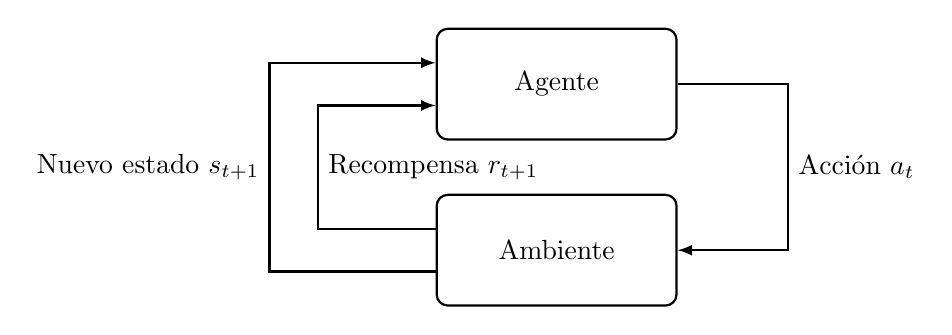
\begin{tikzpicture}[node distance = 6em, auto, thick]
    \node [block] (Agent) {Agente};
    \node [block, below of=Agent] (Environment) {Ambiente};
    
     \path [line] (Agent.0) --++ (4em,0em) |- node [near start]{Acción $a_t$} (Environment.0);
     \path [line] (Environment.190) --++ (-6em,0em) |- node [near start] {Nuevo estado  $s_{t+1}$} (Agent.170);
     \path [line] (Environment.170) --++ (-4.25em,0em) |- node [near start, right] {Recompensa $r_{t+1}$} (Agent.190);
\end{tikzpicture}
	\captionsource{Aprendizaje por reforzamiento}{\fuentePropia}
	\label{fig:decision-tree}
\end{figure}

\subsection{Minería de datos educacional}
La minería de datos utiliza una combinación de bases de conocimientos explícita, conocimientos analíticos complejos y conocimiento de campo para descubrir las tendencias y los patrones ocultos, estas tendencias y patrones forman la base de los modelos predictivos que permiten a los analistas realizar nuevas observaciones de los datos existentes \parencite{luan2002data}. La gran cantidad de información generada hoy en día por los estudiantes permite que la minería de datos obtenga datos relevantes y, a través de métodos estadísticos y otras herramientas relacione la información para conocer si el proceso de enseñanza aprendizaje ha dado resultados positivos. 

\textcite[p.~9]{mining2012enhancing} define la minería de datos educacional (MDE, desde ahora en adelante) como “la teoría que desarrolla métodos, aplica técnicas estadísticas y de aprendizaje automático para analizar los datos recogidos durante el proceso de la enseñanza y aprendizaje” \footnote{\traduccionlibre}. Actualmente, los usos más generales que se le están dando a la MDE básicamente se enfocan en mejorar la estructura del conocimiento y determinar el apoyo pedagógico al estudiante.